% begin module transformations-horizontal-stretches
\begin{frame}\ %
\uncover<1->{}
\psset{xunit=1.4cm, yunit=1.4cm}
\begin{pspicture}(-0.6, -1.4)(6.2,1.4)
\fcAxesStandard{-0.6}{-1.4}{6.2}{1.4}

%Function formula: sin{}(x)
\rput[t](4.71238898, -1.1){\alert<1-2>{$y=sin{}(x)$}}

\uncover<1-2>{
\psplot[linecolor=red, plotpoints=1000]{-0.5}{6}{x 57.29578 mul sin }
}
\uncover<3->{
\psplot[linecolor=blue, plotpoints=1000]{-0.5}{6}{x 57.29578 mul sin }
}

\psline(1.570796327, -0.05)(1.570796327, 0.05)
\rput[t](1.570796327, -0.1) {$\frac{\pi}{2}$}

\psline(3.141592654, -0.05)(3.141592654, 0.05)
\rput[t](3.141592654, -0.1) {$\pi$}


\uncover<3->{
 %Function formula: sin{}(3/2 (x))
\uncover<3>{
\psplot[linecolor=red, plotpoints=1000]{-0.5}{6}{x 1.5 mul 57.29578 mul sin }
}
\uncover<4->{
\psplot[linecolor=blue, plotpoints=1000]{-0.5}{6}{x 1.5 mul 57.29578 mul sin }
}
\rput(3.141592654, -1.1){\alert<3>{$y=\sin{}(cx)$}}

\psline(1.047197551, -0.05)(1.047197551, 0.05)
\rput[t](1.047197551, -0.1) {$\frac{\pi}{2c}$}

\psline(2.094395102, -0.05)(2.094395102, 0.05)
\rput[t](2.094395102, -0.1) {$\frac{\pi}{c}$}

}
\uncover<4->{
\rput[b](3.14,1.1){\alert<4>{$y=\sin\left(\frac{x}{c}\right)$}}
\psplot[linecolor=red, plotpoints=1000]{-0.5}{6}{x 0.666667 mul 57.29578 mul sin }

\psline(2.35619449, -0.05)(2.35619449, 0.05)
\rput[t](2.35619449, -0.1) {$\frac{\pi c}{2}$}

\psline(4.71238898, -0.05)(4.71238898, 0.05)
\rput[t](4.71238898, -0.1) {$\pi c$}
}
\end{pspicture}
%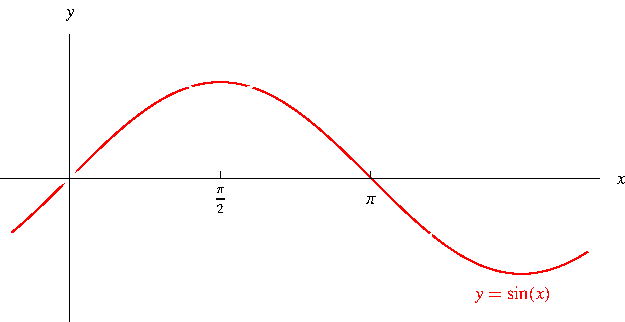
\includegraphics[height=6cm]{precalculus/pictures/01-03-stretcha.pdf}%
%}%
%\only<handout:0| 3>{%
%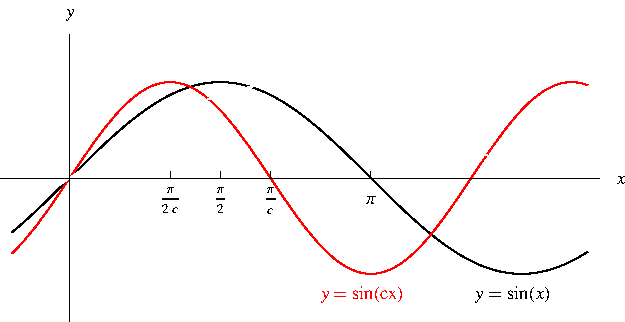
\includegraphics[height=6cm]{precalculus/pictures/01-03-stretchb.pdf}%
%}%
%\only<4->{%
%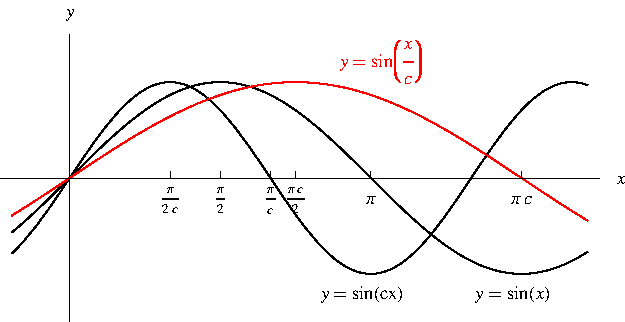
\includegraphics[height=6cm]{precalculus/pictures/01-03-stretchc.pdf}%
%}%a

What happens if we multiply or divide $x$ by a constant $c > 1$ before applying $f$?

\uncover<2->{
\begin{tabular}{|l|l|}
\hline
\alert<handout:0| 3>{$f(cx)$} &%
\uncover<3->{\alert<handout:0| 3>{Compress the graph of $f(x)$ horizontally by a factor of $c$.}} \\%
\alert<handout:0| 4>{$f((1/c)x)$} &%
\uncover<4->{\alert<handout:0| 4>{Stretch the graph of $f(x)$ horizontally by a factor of $c$.}} \\%
\hline
\end{tabular}
}
\end{frame}
% end module transformations-horizontal-stretches
